\section{Results}
%The results contain both the model and a comparison of the model against the alternative approach 
%for that it is the gaol of the model to outperfom the classic technice, not inlcoding neural networks.
%\subsection{Evaluation Of The Model} \label{sec:results_model}
%The trained model, when applied on the test data, shows a final loss of $859.59$ and a mae of $8.43$.
%Since the training process was monitored by the mse rather than the mae, the mse will be the leading factor in this evalulation.
%Mse has been choosen for its abbilty to inlcude outliners more into its error in comparison with mae. This characteristic, in this context, is more desired 
%to surpress abnormalities, i.e. focus on the general increase of confirmed COVID cases.
%\subsection{The Model vs. The Alternativ Approach}
%The model trained for this report and the alternative approach vary in both training concept and results. 
%While the nerual net profits from an test/train split to train on, the least-square-fit-routine is directly applied to the first 
%40 days of the test dataset and thus does not experience the rest of the data.
%The mse of the alternative approach reads $19944936.25$. The figure in \ref{fig:compare} shows the growing deviation of test data towords the end, i.e. the last days, where the exponential function strongly increases with every day.
%For the neural net already knows on how the last 11 days can look like, because it was trained on that with the test and validation set, its error does not increase at a later period.
The results contain both the model and a comparison of the model against the alternative approach. The goal of the model is to outperform the classic technique, not including neural networks.
\subsection{Evaluation Of The Model} \label{sec:results_model}
When the trained model is applied to the test data, it shows a final loss of $859.59$ and a mean absolute error (MAE) of $8.43$. Since the training process was monitored by the mean squared error (MSE) rather than the MAE, the MSE will be the leading factor in this evaluation. MSE has been chosen for its ability to include outliers more into its error in comparison with MAE. This characteristic, in this context, is more desired to suppress abnormalities, i.e. focus on the general increase of confirmed COVID cases.
\subsection{The Model vs. The Alternative Approach}
The model trained for this report and the alternative approach vary in both training concept and results. While the neural net profits from a test/train split to train on, the least-square-fit routine is directly applied to the first 40 days of the test dataset and thus does not experience the rest of the data.
The MSE of the alternative approach reads $19944936.25$. The figure in \ref{fig:compare} shows the growing deviation of test data towards the end, i.e. the last days, where the exponential function strongly increases with every day. For the neural net already knows how the last 11 days can look like, because it was trained on that with the test and validation set, its error does not increase at a later period.



\begin{figure}[H]                          
    \centering
    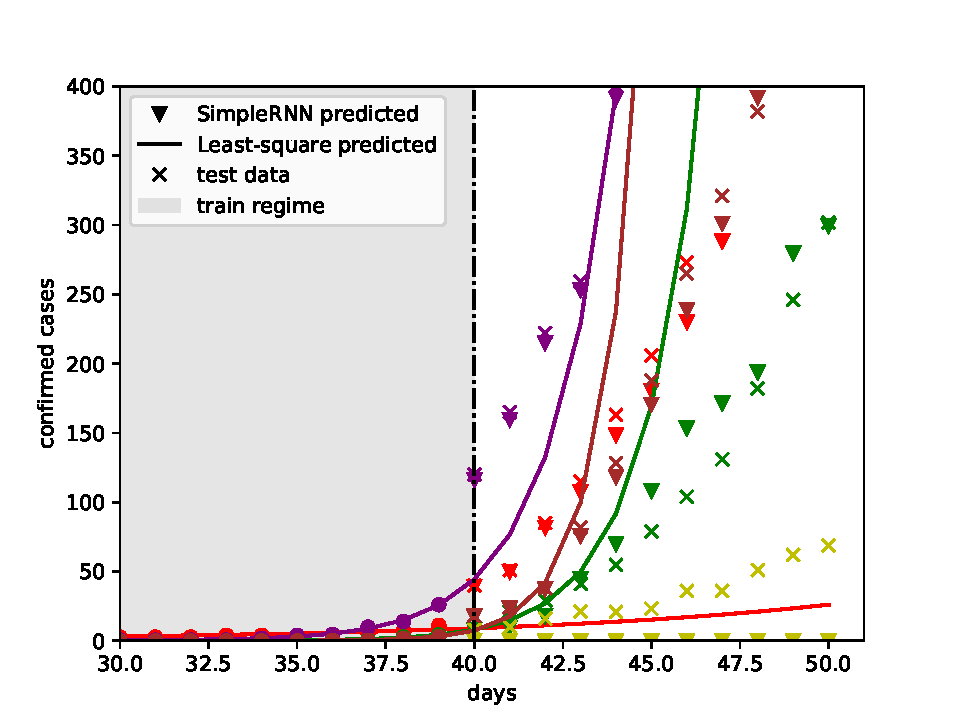
\includegraphics[width = 0.8\textwidth]{images/alternative.pdf}
    \caption{Displayed is a comparison of predictions on confirmed COVID cases between a least square fit routine and a trained neural net. The days are cut to the last 20 days, only including cities where confirmed cases have been found. 
    Two different declarations of confirmed cases are given: SimpleRNN predictions and exponentialy fitted predictions, while the test data is marked with an x. }
    \label{fig:alternative}
\end{figure}


\section{Conclusion}
%For the task, predicting confirmed COVID cases after a given 40 days of data inclding weather informations, the nerual net 
%outperfoms the alternative approach by several magnitudes ($mse_{alternative} = 19944936.25 \quad \to \quad mse_{SimpleRNN} = 859.59)$. \\
%The alternative method haevily relies on the amount of days it is fitted with while the SimpleRNN seemingly 
%knows how to predict a certain coure based on the weather and confirmed cases before the prediction.
%Even tho the neural net perfoms better, it still gets some predictions wrong as can be seen for the yellow case in \ref{fig:alternative}.
%An other approach to the model would be to train the data on a more suffisticated RNN architecture for example \enquote{LSTM}, which would take more time and recources, yet might perfom better on the problem at hand.

For the task of predicting confirmed COVID cases after a given 40 days of data, including weather information, the neural net outperforms the alternative approach by several magnitudes ($mse_{alternative} = 19944936.25 \quad \to \quad mse_{SimpleRNN} = 859.59$).
The alternative method heavily relies on the amount of days it is fitted with, while the SimpleRNN seemingly knows how to predict a certain course based on the weather and confirmed cases before the prediction. Even though the neural net performs better, it still gets some predictions wrong, as can be seen for the yellow case in \ref{fig:alternative}.
Another approach to the model would be to train the data on a more sophisticated RNN architecture, for example, \enquote{LSTM}, which would take more time and resources but might perform better on the problem at hand.